\section{Vektorer} \label{sec:vektorer}
Indtil nu har vi kun set på en endimensionelle bevægelser, men som de fleste ved, sker langt fra alle bevægelser langs en linje. Når en bevægelse foregår i mere end én dimension, beskriver vi positionen med en {\em vektor}.

En vektor er et matematisk objekt, der både har en retning og en størrelse.
Man tegner normalt vektorer som pile, og af denne grund angives de  her som $\va v$, hvor pilen over bogstavet vise, at det er en vektor.
Ligesom man kan lægge tal sammen, kan man også lægge vektorer sammen.
At lægge vektorer sammen svarer til at sætte dem i forlængelse af hinanden,
dvs. at summen af de to vektorer er den vektor, der går fra starten af den ene til slutningen af den anden, når den anden vektor starter ved slutningen af den første. Dette er illustreret på figur \ref{fig:mat:vakadd}, hvilket gør det noget tydeligere, end det er i ord.
Man kan også gange en vektor med et tal (en {\em skalar}), hvilket forlænger eller forkorter vektoren med denne faktor. Ganger man en vektor med $2$, bliver den altså dobbelt så langt, mens den bliver halvt så lang, hvis man ganger den med $1/2$. Det betyder også, at hvis man ganger med en negativ faktor, så vil det ændre både vektorens retning og længde. F.eks. kan man gange en vektor med $-1$, hvilket giver en vektor med samme længde, men hvor retningen er antiparallel til den oprindelige vektor. 
Når vi lægger vektorer sammen eller ganger dem med tal, gælder alle de regneregler vi er vandt til fra de reelle tal (tallene på en tallinje).

\begin{figure} [h!]
    \centering
    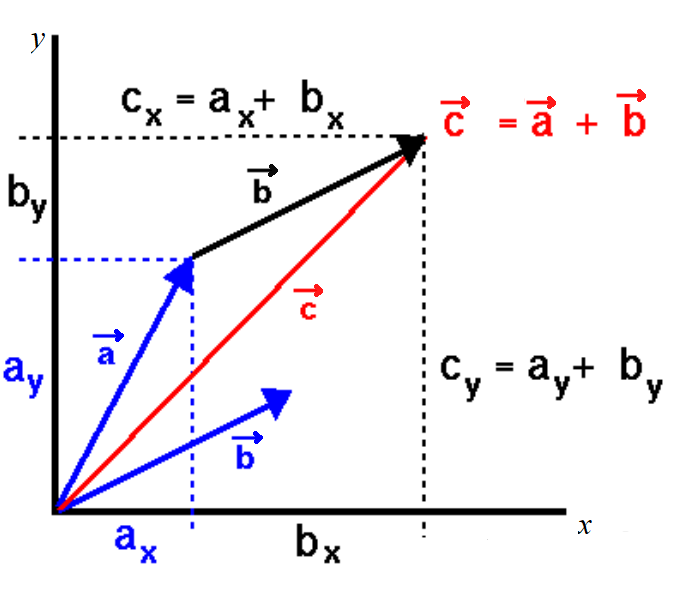
\includegraphics[width = 0.65\textwidth]{Mat/matfig/vektoraddition.png}
    \caption{Illustration af vektoraddition, både grafisk og som komposanter. Baseret på en figur fra {Glenn Reaserach Center} \cite{VectorAddition}.}
    \label{fig:mat:vakadd}
\end{figure}

Når vi arbejder med vektorer i praksis, er det dog typisk ikke vildt brugbart at arbejde med retninger og længder. I stedet splitter man vektorer op i {\em komposanter}, hvilket er en samling af tal, der angiver, hvor langt vektoren peger langs hver af akserne i et koordinat system, se figur \ref{fig:mat:vakadd}. Når man arbejder i to dimensioner, har man altså en $x$-- og $y$--komposant, hvor man i tre dimensioner har en $x$--, $y$-- og $z$--komposant. Kigger vi først på det todimensionelle tilfælde, indfører vi komposantnotationen for vektorer som følger
\begin{equation}
    \va v=\binom{v_x}{v_y} \, ,
\end{equation}
hvor $v_x$ er $x$--komposanten og $v_y$ er $y$--komposanten. Vender vi nu tilbage til at lægge vektorer sammen og gange dem med tal, kan dette nu udtrykkes vha. komposanter. Når man lægger vektorer sammen, som på figur \ref{fig:mat:vakadd}, sker det nemlig komposantvist. Altså har vi at
\begin{equation}
    \va v+\va u=\binom{v_x+u_x}{v_y+u_x} \, .
\end{equation}
Når vi ganger med et tal, er det som at gange ind i en parentes, og alle komposanterne skaleres på samme måde
\begin{equation}
    a\va v=\binom{av_x}{av_y} \, .
\end{equation}

Man skriver normalt længden af en vektor $\va{v}$ som $\abs{\va v}$, men nogle gange skrives blot $v$ hvis man vil være lidt økonomisk med notationen. 
Når man skal finde længden af en todimensional vektor bruges Pythagoras' sætning, hvilket giver os at
\begin{equation}
    \abs{\va v}^2=v^2=v_x^2+v_y^2 \, .\label{pythagoras2}
\end{equation}
I tre dimensioner har vi tilsvarende at
\begin{equation}
    \abs{\va v}^2=v^2=v_x^2+v_y^2+v_z^2 \, .\label{pythagoras3}
\end{equation}

En særlig type af vektorer er dem, hvis længde er 1, og som kaldes \emph{enhedsvektorer}.
Vi skriver dem normalt med en hat, altså $\vu{v}$. Man kan altid danne en enhedsvektor ved at dele vektoren med sin længde\footnote{Når længden ikke er nul.}
\begin{equation}
    \vu v=\frac{\va v}{\abs{\va v}}=\frac{\va v}{v} \, .
\end{equation}
Man kan altså lave en enhedsvektor ud af enhver vektor, men de enhedsvektorer der ligger langs akserne i ens koordinatsystem er særligt interessante.
Disse vektorer kaldes \emph{basisvektorer}, og skrives i tre dimensioner: $\vu{x}$, $\vu{y}$ og $\vu{z}$. I eksplicit komposantnotation er de
\begin{equation}
    \xhat = \begin{pmatrix}
    1\\0\\0 
    \end{pmatrix} \, , \qquad
    \yhat = \begin{pmatrix}
    0\\1\\0 
    \end{pmatrix} \, , \qquad
    \zhat = \begin{pmatrix}
    0\\0\\1 
    \end{pmatrix} \, .
\end{equation}
Det er tit en fordel at skrive en vektor som en skaleret sum af basisvektorer
\begin{equation}
    \va v = v_x \xhat + v_y \yhat + v_z \zhat \, .
\end{equation}
Nu kunne man jo godt spørge sig selv: Når man kan gange vektorer med tal, kan man så gange dem med hinanden?
Svaret er "ja".
Der er faktisk to måder at gøre det på.

Den første er prikproduktet\footnote{Kaldes også for skalarproduktet eller det indre produkt.}, hvor resultatet altid er et tal.
Her ganger man indgangene med hinanden, hvorefter man lægger det hele sammen, så
\begin{equation}\label{mat:prikprodukt}
    \va v\cdot \va u=u_xv_x+u_yv_y+u_zv_z \, .
\end{equation}
Det kaldes også prikproduktet, fordi man angiver det med en prik.
Tager man prikproduktet af en vektor med sig selv, genfinder vi vektorens længde i form af \eqref{pythagoras2} eller \eqref{pythagoras3}.
Mere generelt gælder det at
\begin{equation}
    \abs{\va v\cdot \va u}=\abs{\va v}\abs{\va u}\cos(\theta) \, ,
\end{equation}
hvor $\theta$ er vinkelen imellem de to vektorer, og
$\cos$ står for cosinus, der er en funktion fra trigonometrien.
Har man en retvinklet trekant, er cosinus, for en given vinkel $\theta$, længden af hypotenusen (den længste side) delt med længden af den hosliggende katete (den af de korte sider der danner vinkelen med hypotenusen).
Er vektorerne parallelle, er deres prikprodukt produktet af deres længder, siden $\cos(0^\circ)=1$.
Er vektorerne vinkelrette på hinanden, er prikproduktet nul, da $\cos(90^\circ)=0$.
%Prikproduktet fortæller os således i hvor stor grad to vektorer er vinkelrette, hvilket vi kan bruge til at lave projektioner
%\begin{equation}
%    \text{Proj}_{\va u}(\va v)=\frac{\va v\cdot\va u}{\abs{\va u}^2}\va u=\frac{\va v\cdot\va u}{u^2}\va u
%\end{equation}

Det andet produkt er {\em krydsproduktet}\footnote{Kaldes også for vektorproduktet.},
der er defineret som
\begin{equation} \label{eq:krydsprodukt}
\va{v}\times \va{u}=
    \begin{pmatrix}
    v_x\\v_y\\v_z
    \end{pmatrix}
    \times\begin{pmatrix}
    u_x\\u_y\\u_z
    \end{pmatrix}
    =\begin{pmatrix}
    v_yu_z-v_zu_y\\v_zu_x-v_xu_z\\v_xu_y-v_yu_x
    \end{pmatrix}.
\end{equation}
Modsat prikproduktet giver krydsproduktet kun mening i tre dimensioner, og som det kan ses, er resultatet en ny vektor og ikke et tal.
Grunden til at krydsproduktet er interessant, er at det giver en tredje vektor, der er vinkelret på begge de to første. For at finde retningen af et krydsprodukt bruges højrehåndsreglen, se figur \ref{fig:right_hand_rule_mat}. Den siger, at hvis man lægger pegefingeren langs den første af de to oprindelige vektorer og langefingeren langs den anden, så vil krydsproduktet af de to vektorer ligge i tommelfingerens retning.
\begin{figure}[h!]
    \centering
    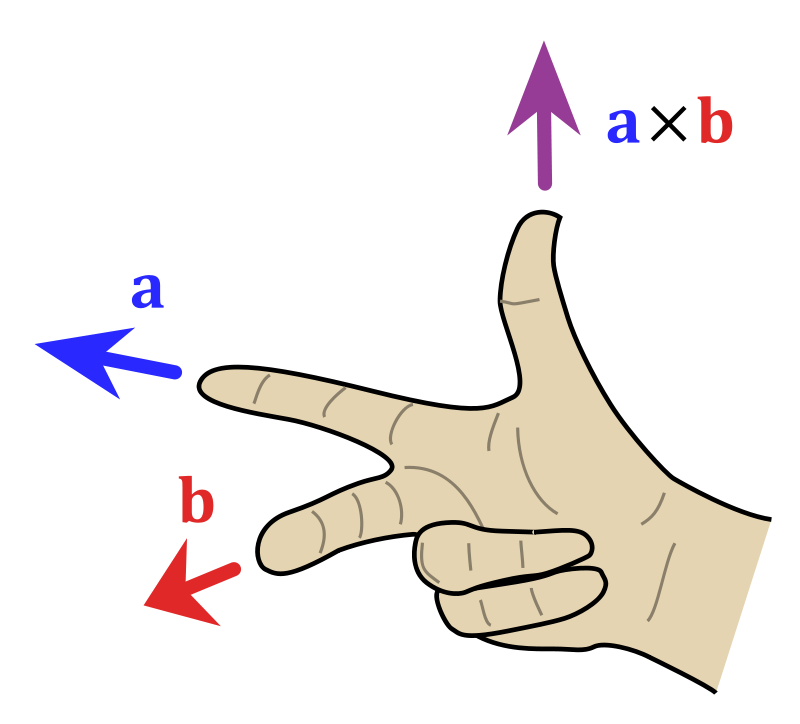
\includegraphics[width = 0.5 \textwidth]{Mat/matfig/righthandmat.png}
    \caption{Højrehåndsreglen. Kilde: \cite{RighthandRuleWikipedia}.}
    \label{fig:right_hand_rule_mat}
\end{figure}

\noindent Længden af et krydsprodukt er
\begin{equation}
    \abs{\va v \times \va u}=\abs{\va v}\abs{\va u}\sin(\theta) \, ,
\end{equation}
hvor $\theta$ er vinklen imellem de to vektorer, og $\sin$ står for sinus, der er en anden trigonometrisk funktion. Hvor cosinus var forholdet imellem hypotenusen og den hosliggende katete, så er sinus forholdet imellem hypotenusen og den modstående katete.
Modsat prikproduktet og almindelig multiplikation har rækkefølgen af de to vektorer i krydsproduktet en indflydelse på resultatet. Bytter man om på de to vektorer skiftes fortegnet.
\begin{equation}\label{eq:krydskommutator}
    \va v \times \va u=-\va u\times \va v \, .
\end{equation}
Ligning \eqref{eq:krydsprodukt} kan være ret besværlig at bruge, så det er ofte lettere at dele udregningen op i basisvektorer. Krydsprodukterne af basisvektorerne er
\begin{subequations}
\begin{align}
    \xhat\times\yhat&=\zhat \, ,\\
    \yhat\times\zhat&=\xhat \, ,\\
    \zhat\times\xhat&=\yhat \, .
\end{align}
\end{subequations}

\newpage

Når vi så skal beskrive den tredimmensionelle bevægelse af et objekt, erstatter vi stedfunktionen $x(t)$ med en stedfunktionsvektor (eller positionsvektor) $\va r(t)$, hvis komposanter hver især opfører sig, præcis som havde det blot været endimensionel bevægelse
\begin{equation}
    \va r(t)=\begin{pmatrix}
    x(t)\\y(t)\\z(t)
    \end{pmatrix} \, .
\end{equation}
For at kunne beskrive mekanik fuldt ud i tre dimensioner, må vi også kigge på differentiation af vektorfunktioner.
For almindelige funktioner var differentialkvotienten hældningen imellem to punkter, når vi lod de to punkter være uendeligt tæt på hinanden
$$
\dv{f}{t}=\lim_{\Delta t\rightarrow 0}\frac{ f(t+\Delta t)- f(t)}{\Delta t} \, .
$$
Der er essentielt tale om en forskel i funktionen $f$ over et kort interval $\Delta t$, så for vektorfunktioner kigger man på en forskel i vektorfunktionen over et kort interval $\Delta t$. Men da forskellen her vil være en differens mellem to vektorer, som jo regnes komposantvis, så må man have at:
\begin{equation}
    \dv{\va r}{t}=\begin{pmatrix} \dd r_x/\dd t\\\dd r_y/\dd t\\\dd r_z/\dd t\end{pmatrix} \, .
\end{equation} 
Nu kan vi skrive Newtons anden lov som
$$
\va F= m\va a=m\dv[2]{\va r}{t} \, ,
$$
hvilket dækker over de tre ligninger
\begin{gather*}
    F_x=ma_x=m\dv[2]{x}{t} \, ,\\
    F_y=ma_y=m\dv[2]{y}{t} \, ,\\
    F_z=ma_z=m\dv[2]{z}{t} \, .
\end{gather*}